%
%%%%%%%%%%%%%%%%%%%%%%%%%%%%%%%%%%%%%%%%%%%%%%%%%%%%%%%%%%%%%%%%%%%%%%%%%%%%%%%%
%
%       KR PACKAGES AND MACROS
%
\documentclass{article}
\pdfpagewidth=8.5in
\pdfpageheight=11in

\usepackage{kr}

% Use the postscript times font!
\usepackage{times}
% \usepackage{soul} % to strikeout, highline, etc.
\usepackage{url}
\usepackage[hidelinks]{hyperref}
\usepackage[utf8]{inputenc}
\usepackage[small]{caption}
\usepackage{graphicx}
\usepackage{amsmath}
\usepackage{amsthm}
\usepackage{booktabs}
\usepackage{algorithm}
\usepackage{algorithmic}
\urlstyle{same}

% the following package is optional:
%\usepackage{latexsym}

% See https://www.overleaf.com/learn/latex/theorems_and_proofs
% for a nice explanation of how to define new theorems, but keep
% in mind that the amsthm package is already included in this
% template and that you must *not* alter the styling.
\newtheorem{example}{Example}
\newtheorem{theorem}{Theorem}

%PDF Info Is REQUIRED.
\pdfinfo{
/TemplateVersion (KR.2022.0, KR.2023.0, KR.2024.0)
}
%
%%%%%%%%%%%%%%%%%%%%%%%%%%%%%%%%%%%%%%%%%%%%%%%%%%%%%%%%%%%%%%%%%%%%%%%%%%%%%%%%
%
%       OUR PACKAGES AND MACROS
%
% \usepackage[
% bibstyle=numeric,
% citestyle=numeric
% ]{biblatex} %Imports biblatex package
% \addbibresource{zugzwang.bib} %Import the bibliography file

\usepackage[x11names]{xcolor}

\usepackage{tikz}
\tikzset{
event/.style={},
smodel/.style={fill=gray!25},
tchoice/.style={draw, circle},
indep/.style={},%{draw, dashed},
proptc/.style = {-latex, dashed},
propsm/.style = {-latex, thick},
doubt/.style = {gray}
}
\usetikzlibrary{calc, positioning, patterns}

\usepackage{hyperref}
\hypersetup{
colorlinks=true,
linkcolor=blue,
citecolor=blue,
urlcolor=blue,
}

\usepackage{commath}
\newtheorem{assumption}{Assumption}
\newtheorem{definition}{Definition}
\newtheorem{proposition}{Proposition}
%\newtheorem{example}{Example}
%\newtheorem{theorem}{Theorem}
\usepackage{amssymb}
\usepackage[normalem]{ulem}
\usepackage{euler}
\usepackage{eucal}
\usepackage[nice]{nicefrac}
\usepackage{stmaryrd}
\usepackage{acronym}
\usepackage{multicol}
\usepackage{cleveref}
\crefname{example}{ex.}{exs.}
\crefname{proposition}{prop.}{props.}
\crefname{assumption}{asp.}{asps.}
%
%   Notation
%
\newcommand{\naf}{\ensuremath{\sim\!}}
\newcommand{\larr}{\ensuremath{\leftarrow}}
\newcommand{\at}[1]{\ensuremath{\!\del{#1}}}
\newcommand{\co}[1]{\ensuremath{\overline{#1}}}
\newcommand{\cla}[1]{\ensuremath{{\cal #1}}}
\newcommand{\clx}[1]{\ensuremath{{\mathbb{#1}}}}
\newcommand{\deft}[1]{\textbf{#1}}
\newcommand{\pset}[1]{\ensuremath{\mathbb{P}\at{#1}}}
\newcommand{\ent}{\ensuremath{\lhd}}
\newcommand{\cset}[2]{\ensuremath{\set{#1,~#2}}}
\newcommand{\langof}[1]{\ensuremath{\cla{L}\at{#1}}}
\newcommand{\uset}[1]{\ensuremath{#1^{\ast}}}
\newcommand{\lset}[1]{\ensuremath{#1_{\ast}}}
\newcommand{\yset}[1]{\ensuremath{\left\langle #1 \right\rangle}}
\newcommand{\stablecore}[1]{\ensuremath{\left\llbracket #1 \right\rrbracket}}
\newcommand{\uclass}[1]{\ensuremath{\intco{#1}}}
\newcommand{\lclass}[1]{\ensuremath{\intoc{#1}}}
\newcommand{\smclass}[1]{\ensuremath{\intcc{#1}}}
\newcommand{\prfunc}{\ensuremath{\mathrm{P}}}
\newcommand{\pr}[1]{\ensuremath{\prfunc\at{#1}}}
\newcommand{\err}[1]{\ensuremath{\mathrm{err}\at{#1}}}
\newcommand{\pw}[1]{\ensuremath{\mu\at{#1}}}
\newcommand{\pwcfname}{\ensuremath{\mu_{\textrm{TC}}}}
\newcommand{\pwc}[1]{\ensuremath{\pwcfname\at{#1}}}
\newcommand{\class}[1]{\ensuremath{[{#1}]_{\sim}}}
\newcommand{\urep}[1]{\ensuremath{\rep{#1}{}}}
\newcommand{\lrep}[1]{\ensuremath{\rep{}{#1}}}
\newcommand{\rep}[2]{\ensuremath{\left\langle #1 \middle| #2 \right\rangle}}
\newcommand{\inconsistent}{\bot}
\newcommand{\given}{\ensuremath{~\middle|~}}
\newcommand{\emptyevent}{\ensuremath{\vartriangle}}
\newcommand{\indepclass}{\ensuremath{\Diamond}}
\newcommand{\probfact}[2]{\ensuremath{#1:#2}}%\newcommand{\probfact}[2]{\ensuremath{#1\mkern-4mu:\mkern-4mu#2}}
\newcommand{\probrule}[3]{\probfact{#1}{#2} \leftarrow #3}
%\newcommand{\tcgen}[1]{\ensuremath{\widehat{#1}}}
\newcommand{\tcgen}[1]{\MODELset\at{#1}}
\newcommand{\lfrac}[2]{\ensuremath{{#1}/{#2}}}
\newcommand{\condsymb}[2]{\ensuremath{p_{#1|#2}}}
%
%   EDIT: fc
%   Added for KR
\newcommand{\ATOMSset}{\ensuremath{\cla{A}}}
\newcommand{\PATOMset}{\ensuremath{\ATOMSset_{\cla{P}}}}
\newcommand{\FACTSset}{\ensuremath{\cla{F}}}
\newcommand{\PROBFset}{\ensuremath{\cla{P}}}
\newcommand{\RULESset}{\ensuremath{\cla{R}}}
\newcommand{\TCHOICEset}{\ensuremath{\cla{T}}}
\newcommand{\MODELset}{\ensuremath{\cla{M}}}
\newcommand{\EVENTSset}{\ensuremath{\cla{E}}}
\newcommand{\CONSISTset}{\ensuremath{\cla{W}}}
%
\newcommand{\conj}{\ensuremath{\wedge}}
\newcommand{\disj}{\ensuremath{\vee}}
\newcommand{\clause}{\ensuremath{\leftarrow}}
%
%
%   Acronyms
%
\acrodef{BK}[BK]{background knowledge}
\acrodef{ASP}[ASP]{answer set program}
\acrodef{NP}[NP]{normal program}
\acrodef{PCR}[PCR]{program with choice rules}
\acrodef{DS}[DS]{distribution semantics}
\acrodef{PF}[PF]{probabilistic fact}%{stochastic choice}%{probabilistic fact}
\acrodef{TC}[TC]{total choice}
\acrodef{SM}[SM]{stable model}
\acrodef{SC}[SC]{stable core}
\acrodef{KL}[KL]{Kullback-Leibler}
\acrodef{SBF}[SBF]{Simple But Fruitful}
\acrodef{RSL}[RSL]{Random Set of Literals}
\acrodef{RCE}[RCE]{Random Consistent Event}
\acrodef{SASP}[SASP]{Stochastic Answer Set Program}
%
%   Reviewing
%
\newcommand{\LOOK}{\ensuremath{\blacksquare}}
\newcommand{\delete}[1]{\xout{#1}}
\newcommand{\franc}[1]{{\color{green!30!black}#1}}
\newcommand{\bruno}{\color{red!60!black}}
\newcommand{\spa}[1]{{\color{brown!80!black}{#1}}}
\newcommand{\dietmar}[1]{{\color{brown!40!black}#1}}

\newcounter{remark}
\newcommand{\remark}[2]{%
	\stepcounter{remark}%
	\!{\color{red}/\!}%
	#1%
	{\!\color{red}/}\footnotemark[\arabic{remark}]%
	\footnotetext[\arabic{remark}]{{\color{red}/}#2}%
	}
\newcommand{\note}[1]{
	\stepcounter{remark}%
	{\!\!\color{red}/}\footnotemark[\arabic{remark}]\!\!%
	\footnotetext[\arabic{remark}]{{\color{red}/}#1}
}
%
%%%%%%%%%%%%%%%%%%%%%%%%%%%%%%%%%%%%%%%%%%%%%%%%%%%%%%%%%%%%%%%%%%%%%%%%%%%%%%%%
%
%   PREAMBLE / METADATA
%
\title{% \textbf{KR - Formal improvement}
  An Algebraic Approach to Stochastic ASP}

% Single author syntax
\iffalse % (remove the multiple-author syntax below and \iffalse ... \fi here)
\author{%
	Author name
	\affiliations
	Affiliation
	\emails
	email@example.com    % email
}
\fi
% Multiple author syntax
\author{%
Francisco Coelho$^{1,2}$\and
Bruno Dinis$^{1,3}$\and
Dietmar Seipel$^4$\and
Salvador Abreu$^{1,2}$\\
\affiliations
$^1$University of Évora\quad
$^2$NOVA LINCS\quad
$^3$CIMA\quad
$^4$Universit\"at W\"urzburg
\emails
\texttt{\{fc, bruno.dinis, spa\}@uevora.pt dietmar.seipel@uni-wuerzburg.de}
}

\pagestyle{plain}

\begin{document}

\maketitle

\begin{abstract}
  We address the problem of extending probability from the total
  choices of an \acs{ASP} program to the \aclp{SM}, and from there to
  general events. %
  \spa{lengthen abstract}
  % 
  Our approach is algebraic in the sense that it relies on an
  equivalence relation over the set of events and uncertainty is
  expressed with variables and polynomial expressions.
  % 
  We illustrate our methods with two examples, one of which shows a
  connection to bayesian networks.
\end{abstract}
%%%%%%%%%%%%%%%%%%%%%%%%%%%%%%%%%%%%%%%%%%%%%%%%%%%%%%%%%%%%%%%%%%%%%%%%%%%%%%%%
%
%   PAPER START
%
%
%
\section{Introduction and Motivation}
%
%
%
A major limitation of logical representations in real world
applications is the implicit assumption that the \acl{BK} is perfect.
This assumption is problematic if data is noisy, which is often the
case.  Here we aim to explore how \acl{ASP} programs with
probabilistic facts can lead to characterizations of probability
functions on the program's domain, which is not straightforward in the
context of \acl{ASP}, as explained below (see also
\cite{verreet2022inference,pajunen2021solution,cozman2020joy,baral2009probabilistic}).
Unlike current systems such as ProbLog \cite{de2007problog}, P-log
\cite{baral2009probabilistic} or LP\textsuperscript{MLN}
\cite{lee2016weighted}, that derive a probability distribution from a
program, in our system some choices are represented by a parameter
that can be later estimated from further information, \emph{e.g.}\
observations.  This approach enables later refinement and scoring of a
partial program of a model from additional evidence.

% \note{Maybe add a sentence explaining the main idea about ASP and
% why/what for is it interesting/useful?}
\Ac{ASP} \cite{lifschitz2002answer,lifschitz2008twelve} is a logic
programming paradigm based on the \ac{SM} semantics of \acp{NP}.
\Ac{ASP} programs represent a problem and the resulting models
(\emph{answer sets}) can be found using the latest advances in SAT
solving technology
\cite{gebser2011potassco,adrian2018asp,niemela1997smodels} or through
top-down searching
\cite{alberti2017cplint,arias2020justifications,marple2017computing}.
Unlike Prolog, \ac{ASP} is a truly declarative language that supports
language constructs such as disjunction in the head of a rule, choice
rules, and both hard and weak constraints.
%
%
The \ac{DS} \cite{sato1995statistical,riguzzi2022foundations} is a key
approach to extend logical representations with probabilistic
reasoning.

%
%   BEGIN EDIT: fc
%   Syntax and Semantics
%
%%%

%%%
% \franc{Begin: Syntax and Semantics - move to (new) section 2}
%{\bruno I think that Syntax and Semantics deserves a separate (sub)section}
%%%

%%%
%
%   END EDIT: fc
%   Syntax and Semantics
%
%

We can foresee two key applications of this extended probability:
\begin{enumerate}
\item Support probabilistic reasoning/tasks on the program domain,
  \textit{i.e.} the set of all events, $\EVENTSset$.
\item Given a dataset and a divergence measure, the program can be
  scored (by the divergence w.r.t.\ the \emph{empiric} distribution of
  the dataset), and weighted or sorted amongst other programs.  These
  are key ingredients in algorithms searching, for example, optimal
  models of a dataset.
\end{enumerate}

\franc{\LOOK~Stress propagation of probabilities.} To extend probabilities from \aclp{TC} we start with the stance that
\emph{a program describes an observable system}, that \emph{the
  \aclp{SM} are all the possible states} of that system and that
\emph{observations (i.e.\ events) are stochastic} --- one observation
can be sub-complete (a proper subset of a \ac{SM}) or super-complete
(a proper superset of a \ac{SM}),
%\note{We should explain this!}
and might not determine the real state of the system.  From here,
probabilities must be extended from \acp{TC} to \acp{SM} and then to
any event. \franc{\LOOK~State that we are propagating from the models, not the programs.}
%
This extension process starts with a critical problem, illustrated by
the example in \cref{sec:example.1}, concerning situations where
multiple \acp{SM}, $ab$ and $ac$, result from a single \ac{TC}, $a$,
but there is not enough information (in the program) to assign a
single probability to each \ac{SM}.  We propose to address this issue
by using algebraic variables to describe that lack of information and
then estimate the value of those variables from empirical data.  This
lack of uniqueness is also addressed in \cite{cozman2020joy} along a
different approach, using credal sets.

In another related work \cite{verreet2022inference} epistemic
uncertainty (or model uncertainty) is considered as a lack of
knowledge about the underlying model, that may be mi\-ti\-ga\-ted via
further observations.  This seems to presuppose a bayesian approach to
imperfect knowledge in the sense that having further observations
allows to improve/correct the model.  Indeed, that approach uses Beta
distributions on the total choices in order to be able to learn a
distribution on the
events. %\remark{events}{Check this: do they learn distributions on the events?}
This approach seems to be specially fitted to being able to tell when
some probability lies beneath some given value.  Our approach seems to
be similar in spirit, while remaining algebraic in the way that the
extension of probabilities is addressed.

The example in \cref{sec:example.1} uses the code available in the
project's
repository\footnote{\url{https://git.xdi.uevora.pt/fc/sasp}},
developed with the \textit{Julia} programming language
\cite{bezanson2017julia}, and the \textit{Symbolics}
\cite{gowda2021high} libraries.
%
%

\section{Syntax and Semantics of Stochastic \ac{ASP}}
%%%

\franc{\LOOK~Underline that the scope of this syntax is just to start studying our propagation method.}

We start this overview with the syntax and \ac{ASP} semantics of
(propositional) \aclp{NP} and then proceed to the case of
probabilistic annotations.

%%%
%\textbf{Valid Normal programs.} 
Let $\ATOMSset$ be a finite set.  A \textit{positive literal}, or
\textit{atom}, is any $a \in \ATOMSset$ and a \textit{negative
  literal} is $\neg a$, also denoted $\co{a}$, for $a\in\ATOMSset$.  A
\textit{literal} is a positive or a negative literal.  A \textit{fact}
is a literal.  For literals $x_1, \ldots, x_n$, a \emph{conjunction}
is $x_1 \conj \cdots \conj x_n$ and a \textit{disjunction} is
$x_1 \disj \cdots \disj x_n$.  A \textit{normal rule} is $h \clause b$ where
$h$ is a literal, the \textit{head}, and $b$ a conjunction, the
\textit{body}. In a \textit{choice rule} the head is a disjunction. An \textit{\acf{ASP}} is a set of facts and (both normal and choice) rules,
denoted, resp.  $\FACTSset\at{P}, \RULESset\at{P}$,  or simply $\FACTSset, \RULESset$. \franc{\LOOK~Notice that choice rules can be converted to a normal rules \cite{gebser2022answer}.}
%
% Semantics of Normal Programs

The semantics of an \ac{ASP} can have different definitions
\cite{lifschitz2008twelve}.  A common definition is as follows
\cite{gelfond1988stable}.  Let $P$ be a \acl{NP}.  The \emph{reduct}
of $P$ relative to the set of atoms $X$ results from (i) deleting
rules that contains a literal $\neg x$ with $x \in X$ and then (ii)
deleting literals $\neg y$ from the bodies of the remaining rules.
Now, $\MODELset\at{P}$, or simply $\MODELset$, is a \acf{SM} of $P$ if it is the minimal model of the reduct
of $P$ relative to $\MODELset$.

%
%   EDIT: fc
%   stable models without grounding
Another promising approach to handle the generation of stable mo\-dels is the
one supported by \texttt{s(CASP)}, a system that can evaluate ASP
programs with function symbols (functors) and constraints without
grounding them either before or during execution, using a method
similar to SLD resolution
\cite{marple2017computing,arias2020justifications}.  This enables the
generation of human readable explanations of the results of programs
and addresses two major issues of grounding-based solvers, that 1)
either do not support function symbols or, using finite domains, lead
to exponential groundings of a program and 2) compute the complete
model of the grounded program when, in some scenarios, it is desirable
to compute only a partial stable model containing a query.

% Syntax of SAPS
\emph{\Acfp{SASP}} extend \ac{ASP} by adding facts with probabilistic
annotations: A \textit{\ac{PF}} is $\probfact{a}{p}$ where $a$ is an
atom and $p\in\intcc{0,1}$.  We denote the set of \aclp{PF} of a
program by $\PROBFset$, and $\PATOMset$ the set of positive literals
in $\PROBFset$. \franc{\LOOK~Relate to \cite{kifer1992theory} and state that our propagation of probability is through the models of the program, not its syntax.}

%
%\textbf{Interpretation of SASP programs.} 
The \emph{derived program} of a \ac{SASP} is obtained by replacing
each \acl{PF} $\probfact{a}{p}$ by $a \disj \co{a}$.  The \textit{\aclp{SM}} of a
\acs{SASP} program are the \aclp{SM} of its derived program. The set
of \acp{SM} of a (derived or) \acs{SASP} program is denoted
$\MODELset$.

An \emph{event} is a set of literals.  We denote the set of events by
$\EVENTSset$.  For $e \in \EVENTSset$, if there exists a positive
literal $x$ such that $\set{x, \co{x}} \subseteq e$ then $e$ is
\textit{inconsistent}; otherwise $e$ is \textit{consistent}.  The set
of consistent events is denoted by $\CONSISTset$.

%\textbf{Probability of total choices.} 
A disjunctive head $a \disj \co{a}$ in the derived program represents
a single \textit{choice}, either $a$ or $\co{a}$.  A \textit{\acl{TC}}
of the derived program, and of the SASP program, is
$t = \set{a' \given \probfact{a}{p} \in \PROBFset}$ where each $a'$ is
either $a$ or $\co{a}$.  We denote $\TCHOICEset$ the set of total
choices of a \ac{SASP} or derived program.  The \emph{probability of
  the \acl{TC} $t \in \TCHOICEset$} is
\begin{equation}
	\pr{T = t} = 
	\prod_{\substack{
		\probfact{a}{p}~ \in ~\PROBFset,\\
		a~ \in~ t}} p 
	\prod_{\substack{
		\probfact{a}{p}~ \in ~\PROBFset,\\
		\co{a}~\in~ t}} \co{p}
	\label{eq:prob.total.choice}
\end{equation}

where $T$ is a random variable whose values are \aclp{TC}.

Some \aclp{SM} are entailed from some \aclp{TC} while other \acp{SM}
are entailed by other \acp{TC}.  We write $\tcgen{t}$ to represent the
set of \acp{SM} entailed by $t \in \TCHOICEset$.
%
%%%%%%%%%%%%%%%%%%%%%%%%%%%%%%%%%%%%%%%%%%%%%%%%%%%%%%%

\franc{\textbf{BEGIN} other approaches and systems.}

%%%%%%%%%%%%%%%%%%%%%%%%%%%%%%%%%%%%%%%%%%%%%%%%%%%%
%
%   EDIT: fc
%   Cozman's credal sets
A related approach to define semantics of normal programs with
probabilistic facts is described in \cite{cozman2020joy}, where
$\pr{T = t}$ is defined like in \cref{eq:prob.total.choice} but then,
for $a \in \ATOMSset$, $\pr{a \given t}$ is unknown but bounded by
$\underbar{\prfunc}\at{a \given t}$ and
$\overline{\prfunc}\at{a \given t}$, that can be explicitly estimated
from the program.
%

%

\begin{itemize}
	\item P-Log \franc{still missing}.
	\item \franc{draft:}~Problog2: \cite{fierens2015inference,verreet2022inference}.  
	\begin{itemize}
	\item A ProbLog program specifies a probability distribution over
	  possible worlds.
	\item world is a model of $C \cup R$ where $C$ is a total choice
	  and $R$ the set of rules of a program.
%% check out references...    
	\item Semantics only defined for \textit{sound} programas {\bruno
		(Riguzzi and Swift 2013)} i.e., programs for which each
	  possible total choice $C$ leads to a well-founded model that is
	  two-valued or `total' {\bruno (Riguzzi and Swift 2013; Van
		Gelder et al. 1991)}.  A sufficient condition for this is that
	  the rules in the ProbLog program are locally stratified {\bruno
		(Van Gelder et al. 1991)}.  In particular, this trivially
	  holds for all negation-free programs.
	\item Probability of a possible world that is a model of the
	  program is the probability of the total choice.  Otherwise
	  probability is 0.
	\end{itemize}
  \item \franc{draft:}~$LP^{MLN}$: \cite{lee2016weighted,lee2017lpmln}
	\begin{itemize}
	\item Extends Problog
	\item based on Markov Logic (Richardson and Domingos 2006)
	\item weighted rules $a \leftarrow b, n$ where $a$ is disjunction
	  of atoms, $b$ is conjunction of atoms, $n$ is constructed from
	  atoms using conjunction, disjunction and negation.
	\item For each model there is a unique maximal set of rules that
	  are satisfied by it.  The respective weights determine the
	  probability of the model.
	\end{itemize}
\end{itemize}
%
%%%%%%%%%%%%%%%%%%%%%%%%%%%%%%%%%%%%%%%%%%%%%%%%

\franc{\textbf{END} other approaches and systems.}

%%%%%%%%%%%%%%%%%%%%%%%%%%%%%%%%%%%%%%%%%%%%%%%%
%
\franc{\LOOK~Our goal} is to extend the probability $\pr{T = t}$ in
\cref{eq:prob.total.choice} (which is, indeed, a product of Bernoulli
distributions \cite{Teugels90}), from \aclp{TC} to the program's
events, $\pr{E = e}$.
%%%


% Let $\ATOMSset$ be a finite set of atoms.  A \emph{pre-total choice}
% is a subset $t^{\ast}$ of \ATOMSset.  The \emph{\acl{TC}} (TC)
% associated to $t^{\ast}$ is the set $t := t^{\ast} \cup \set{\co{a}
% \given a \in \ATOMSset \setminus t^{\ast}}$ where $\co{a}$ stands
% for $\neg a$.  \Acp{PF} are the most basic \ac{DS} stochastic
% primitives and take the form  $\probfact{a}{p}$ where each
% $a\in\ATOMSset$ is associated to some $p\in\intcc{0, 1}$.  Each
% \ac{PF} then represents a boolean random variable that is true with
% probability $p$ and false with probability $\co{p} = 1 - p$. 

% % \note{revisit this part.  $\co{a}$ não foi definido! Talvez
% % escrever $\neg a$ na definição de $t$?}
% Let $F = \set{\probfact{a}{p} \given a \in \ATOMSset, p \in \intcc{0, 1}}$.  For a \acl{TC} $t$ over $\ATOMSset$, define
% $$
% \begin{aligned}
%     P_t :=  &\set{ p \given a \in t^{\ast} \wedge \probfact{a}{p} \in F} \\
%         \cup  &\set{\co{p} \given a \in t \setminus t^{\ast} \wedge \probfact{a}{p} \in F}
% \end{aligned}
% $$

% and

% \begin{equation}
%     \pr{T = t} = \prod_{p \in P_t} p,
%     \label{eq:prob.total.choice}
% \end{equation}

% where $T$ is a random variable whose values are \aclp{TC}.
%%%
%\franc{End: Syntax and Semantics}

%
%
%
\section{A Simple but Fruitful Example}\label{sec:example.1}
%
%
%
In this section we consider a somewhat simple example that showcases
the problem of extending probabilities from \aclp{TC} to \aclp{SM} and
then to events.  As mentioned before, the main issue arises from the
lack of information in the program to assign a single probability to
each stable model.  This becomes a crucial problem in situations where
multiple \aclp{SM} result from a single \acl{TC}.  We will come back
to this example in \cref{subsec:sbf.example}, after we present our
proposal for extending probabilities from \aclp{TC} to \aclp{SM} in
\cref{sec:extending.probalilities}.


\begin{example}\label{running.example}
	Consider the program
	\begin{equation}
		\begin{aligned}
			\probfact{a&}{0.3} ,\cr
			b \vee c          & \leftarrow a.
		\end{aligned}
		\label{eq:example.1}
	\end{equation}
	% {\bruno Explain the notation $ab$}
	The \aclp{SM} of this \ac{SASP} are the ones from its derived
	program: $\co{a}, ab$ and $ac$.  We use short-hand expressions
	like $ab$ to denote \textit{e.g.} the set $\set{a, b}$.  While it
	is straightforward to assume $\pr{\co{a}}=0.7$, there is no
	obvious explicit way to assign values to $\pr{ab}$ and $\pr{ac}$.
	Instead, we can use a parameter $\theta$ as in
	$$
	\begin{aligned}
	  \pr{ab} & = 0.3 \theta,\cr
				\pr{ac} & = 0.3 (1 - \theta)
	\end{aligned}
	$$
	to express our knowledge that $ab,ac$ are events related in a
	certain way and, simultaneously, our uncertainty about that
	relation.  The pa\-ra\-me\-ter $\theta=\theta_{s,t}$ depends on
	both the \acl{SM} $s$ and the \acl{TC} $t$.  This uncertainty can
	then be addressed with the help of adequate distributions, such as
	empirical distributions from datasets.
\end{example}

If an \ac{ASP} program is intended to describe some system then:

\begin{enumerate}

\item With a probability set for the \aclp{SM}, we want to extend it
  to all the events of the program domain.

\item In the case where some statistical knowledge is available, for
  example, in the form of a distribution, we consider it as
  ``external'' knowledge about the parameters, that doesn't affect the
  extension procedure described below.

\item Statistical knowledge can be used to estimate parameters and to
  ``score'' the program.

\item\label{item:program.selection} If that program is only one of
  many possible candidates then that score can be used, \emph{e.g.} as
  fitness, by algorithms searching (optimal) programs of a dataset of
  observations.

\item If observations are not consistent with the program, then we
  ought to conclude that the program is wrong and must be changed
  accordingly.
\end{enumerate}

Currently, we are addressing the problem of extending a probability
function (possibly using parameters such as $\theta$ above), defined
on the \acp{SM} of a program, to all the events of that program.  This
extension must satisfy the Kolmogorov axioms of probability so that
probabilistic reasoning is consistent with the \ac{ASP} program and
follow our interpretation of \aclp{SM} as the states of an observable
system.

As sets, the \acp{SM} can have non-empty intersection.  But, as states
of a system, we assume that \acp{SM} are disjoint events, in the
following sense:

\begin{assumption}\label{assumption:smodels.disjoint}
  \Aclp{SM} are disjoint events: For any set $X$ of \aclp{SM},
  \begin{equation}
	\pr{X} = \sum_{s\in X}\pr{s}
  \end{equation}
\end{assumption}

Consider the \aclp{SM} $ab, ac$ from \cref{running.example}, that
result from the rule $b \vee c \leftarrow a$ and the \acl{TC}
$\set{a}$.  Since we intend to associate each \acl{SM} with a state of
the system, $ab$ and $ac$ should be \emph{disjoint} events.  So
$b \vee c$ is interpreted as an \emph{exclusive disjunction} and, from
that particular rule, no further relation between $b$ and $c$ is
assumed.  This does not prevent that other rules may be added that
entail further dependencies between $b$ and $c$, which in turn may
change the \aclp{SM}.

By not making distribution assumptions on the rules of the program we
can state such properties on the semantics of the program, as we've
done in assumption \ref{assumption:smodels.disjoint}.
%
%
%
\section{Extending Probabilities}\label{sec:extending.probalilities}
%
%
%
\begin{figure}[t]
	\begin{center}
		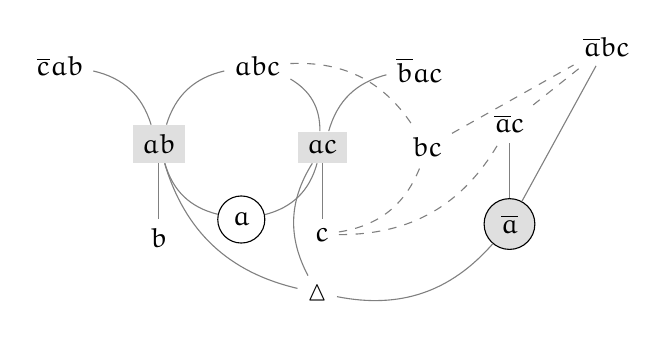
\begin{tikzpicture}[node distance=2em]
			\node[event] (E) {$\emptyevent$};
			\node[tchoice, above left = of E] (a) {$a$};
			\node[smodel, above left = of a] (ab) {$ab$};
			\node[smodel, above right = of a] (ac) {$ac$};
			\node[event, below = of ab] (b) {$b$};
			\node[event, below = of ac] (c) {$c$};
			\node[event, above right = of ab] (abc) {$abc$};
			\node[event, above left = of ab] (abC) {$\co{c}ab$};
			\node[event, above right = of ac] (aBc) {$\co{b}ac$};
			\node[indep, right = of ac] (bc) {$bc$};
			\node[tchoice, smodel, below right = of bc] (A) {$\co{a}$};
			\node[event, above = of A] (Ac) {$\co{a}c$};
			\node[event, above right = of Ac] (Abc) {$\co{a}bc$};
			% ----
			\draw[doubt] (a) to[bend left] (ab);
			\draw[doubt] (a) to[bend right] (ac);

			\draw[doubt] (ab) to[bend left] (abc);
			\draw[doubt] (ab) to[bend right] (abC);

			\draw[doubt] (ac) to[bend right] (abc);
			\draw[doubt] (ac) to[bend left] (aBc);

			\draw[doubt, dashed] (Ac) to (Abc);

			\draw[doubt] (A) to (Ac);
			\draw[doubt] (A) to (Abc);

			\draw[doubt] (ab) to[bend right] (E);
			\draw[doubt] (ac) to[bend right] (E);
			\draw[doubt] (A) to[bend left] (E);

			\draw[doubt] (ab) to (b);
			\draw[doubt] (ac) to (c);
			% \draw[doubt] (ab) to[bend left] (a);
			% \draw[doubt] (ac) to[bend right] (a);
			\draw[doubt, dashed] (c) to[bend right] (bc);
			\draw[doubt, dashed] (abc) to[bend left] (bc);
			\draw[doubt, dashed] (bc) to (Abc);
			\draw[doubt, dashed] (c) to[bend right] (Ac);
		\end{tikzpicture}
	\end{center}

	\caption{Some events related to the \aclp{SM} of
	  \cref{running.example}.  The circle nodes are \aclp{TC} and
	  shaded nodes are \aclp{SM}.  Solid lines represent relations
	  with the \acp{SM} and dashed lines some sub-set relations with
	  other events.  The set of events contained in all \aclp{SM},
	  denoted by $\emptyevent$, is empty in this example. \franc{Consider denoting the event $\emptyset$ by $\lambda$ and using $\Lambda$ instead of $\emptyevent$. We still need to denote the set of events related with all the \acp{SM}, but we are being less confusing with this notation.}}
	\label{fig:running.example}
\end{figure}

The diagram in \cref{fig:running.example} illustrates the problem of
extending probabilities from \aclp{TC} to \aclp{SM} and then to
general events in an \emph{edge-wise} process, where the value in a
node is defined from the values in its neighbors.  This quickly leads
to coherence problems concerning probability, with no clear systematic
approach.  Notice that $bc$ is not directly related with any \acl{SM}
therefore propagating values through edges would assign a hard to
justify ($\not= 0$) value to $bc$.  Instead, we propose to base the
extension in the relation an event has with the \aclp{SM}.
%
%
%
\subsection{An Equivalence Relation}\label{subsec:equivalence.relation}
%
%
%
\begin{figure}[t]
	\begin{center}
		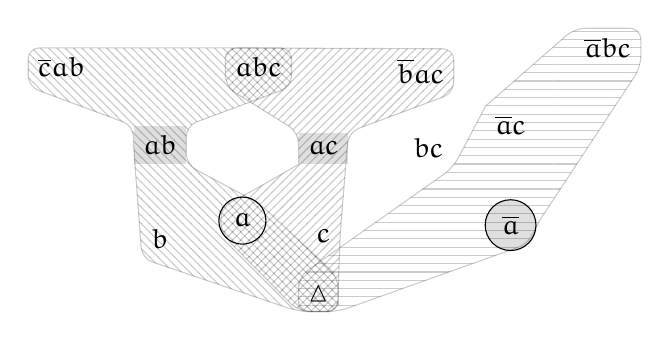
\begin{tikzpicture}[node distance=2em]
			\node[event] (E) {$\emptyevent$};
			\node[tchoice, above left = of E] (a) {$a$};
			\node[smodel, above left = of a] (ab) {$ab$};
			\node[smodel, above right = of a] (ac) {$ac$};
			\node[event, below = of ab] (b) {$b$};
			\node[event, below = of ac] (c) {$c$};
			\node[event, above right = of ab] (abc) {$abc$};
			\node[event, above left = of ab] (abC) {$\co{c}ab$};
			\node[event, above right = of ac] (aBc) {$\co{b}ac$};
			\node[indep, right = of ac] (bc) {$bc$};
			\node[tchoice, smodel, below right = of bc] (A) {$\co{a}$};
			\node[event, above = of A] (Ac) {$\co{a}c$};
			\node[event, above right = of Ac] (Abc) {$\co{a}bc$};
			% ----
			\path[draw, rounded corners, pattern=north west lines, opacity=0.2]
			(ab.west) --
			(ab.north west) --
			%
			(abC.south west) --
			(abC.north west) --
			(abC.north) --
			%
			(abc.north east) --
			(abc.east) --
			(abc.south east) --
			%
			(ab.north east) --
			(ab.east) --
			(ab.south east) --
			%
			(a.north east) --
			%
			(E.north east) --
			(E.east) --
			(E.south east) --
			(E.south) --
			(E.south west) --
			%
			(b.south west) --
			%
			(ab.west)
			;
			% ----
			\path[draw, rounded corners, pattern=north east lines, opacity=0.2]
			(ac.south west) --
			(ac.west) --
			(ac.north west) --
			%
			(abc.south west) --
			(abc.west) --
			(abc.north west) --
			%
			(aBc.north east) --
			(aBc.east) --
			(aBc.south east) --
			%
			(ac.north east) --
			%
			(c.east) --
			%
			(E.east) --
			(E.south east) --
			(E.south) --
			(E.south west) --
			%
			(a.south west) --
			(a.west) --
			(a.north west) --
			(a.north) --
			%
			(ac.south west)
			;
			% ----
			\path[draw, rounded corners, pattern=horizontal lines, opacity=0.2]
			% (A.north west) --
			%
			(Ac.north west) --
			%
			(Abc.north west) --
			(Abc.north) --
			(Abc.north east) --
			(Abc.south east) --
			%
			% (Ac.north east) --
			% (Ac.east) --
			%
			(A.east) --
			(A.south east) --
			%
			(E.south east) --
			(E.south) --
			(E.south west) --
			(E.west) --
			(E.north west) --
			%
			(bc.south east) --
			%
			(Ac.north west)
			;
		\end{tikzpicture}
	\end{center}

	\caption{Classes of (consistent) events related to the \aclp{SM}
	  of \cref{running.example} are defined through intersections and
	  inclusions.  In this picture we can see, for example, the
	  classes $\set{\co{c}ab, ab, b}$ and $\set{a, abc}$.  Different
	  fillings correspond to different classes and, as before, the
	  circle nodes are \aclp{TC} and shaded nodes are \aclp{SM}.
	  Notice that $bc$ is not in a shaded area.}
	\label{fig:running.example.classes}
\end{figure}

\franc{\LOOK~Should we bring back the parts moved to the appendix?}

% Given an ASP program, we consider a set of \emph{atoms}
% $ \ATOMSset$, the set $\cla{L}$ of the \emph{literals} over
% \ATOMSset, and the set of \emph{events} $\EVENTSset$ such that
% $e \in \EVENTSset \clause e \subseteq \cla{L}$.  We also consider
% $\CONSISTset$ the set of \emph{worlds} (consistent events),
% %\note{Be more precise on this definition} 
% a set of \emph{\aclp{TC}} $\TCHOICEset$ such that for every $a \in \ATOMSset$ we have $a \in t$ or $\neg a \in t$
% %\note{Shouldn't it be $a \in t$ or $\neg a \in t$???}
% , and $\PROBFset$ the set of \emph{\aclp{SM}} such that $ \PROBFset\subset\CONSISTset$.  At last, the set of \aclp{SM} entailed by the \acl{TC} $t$ is denoted by $\tcgen{t}$.
%
%%%%%%%%%%%%%%%%%%%%%%%%%%%%%%%%%%%%%%%%%%%%%%%%%%%%%%%%%%%%%%%%%%%%%%
%

\franc{\textbf{BEGIN}~Draft zone to integrate with \cite{kifer1992theory}}
%

We need to \franc{define a lattice $\clx{T}$} of ``truth values'' to \franc{interpret any event} as an \franc{ideal}. And do so in a way compatible with \cite{kifer1992theory}. 


And \textit{families $\clx{F}_i:\clx{T}^i \to \clx{T}$ of total continuous computable functions} to define \textbf{term-}annotated clause heads \franc{Maybe we don't need this \textbf{now}}; we are considering only c-annotations.

\franc{\textbf{END}~Draft zone to integrate \cite{kifer1992theory}}
%
%%%%%%%%%%%%%%%%%%%%%%%%%%%%%%%%%%%%%%%%%%%%%%%%%%%%%%%%%%%%%%%%%%%%%%
%

Our path to extend probabilities starts with a perspective of
\aclp{SM} as playing a role similar to \emph{prime factors}\franc{~or \emph{principal ideals}}.  The
\aclp{SM} of a program are the irreducible events entailed from that
program and any event must be considered under its relation with the
\aclp{SM}.

From \cref{running.example} and \cref{fig:running.example.classes}
consider the \acp{SM} $\co{a}, ab, ac$ and events $a, abc$ and $c$.
While $a$ is related with (contained in) both $ab, ac$, the event $c$
is related only with $ac$.  So, $a$ and $c$ are related with different
\acp{SM}.  On the other hand, $abc$ contains with both $ab, ac$.  So
$a$ and $abc$ are related with the same \aclp{SM}.

%Recall that $\MODELset$ is the set of \aclp{SM}.
\begin{definition}\label{def:stable.core}
	The \textit{\ac{SC}} of the event $e\in \EVENTSset$ is
	\begin{equation}
		\stablecore{e} := \set{s \in \MODELset \given s \subseteq e \vee e \subseteq s}. \label{eq:stable.core}
	\end{equation}
	% where $\MODELset$ is the set of \aclp{SM}.
\end{definition}

We now define an equivalence relation so that two events are related
if either both are inconsistent or both are consistent and, in the
latter case, with the same \acl{SC}.

\begin{definition}\label{def:equiv.rel}
  For a given program, let $u, v \in \EVENTSset$.  The equivalence
  relation $\sim$ is defined by
	\begin{equation}
		u \sim v : \leftarrow u,v \not\in\CONSISTset \vee \del{u,v \in \CONSISTset \wedge \stablecore{u} = \stablecore{v}}.\label{eq:equiv.rel}
	\end{equation}
\end{definition}

Observe that the minimality of \aclp{SM} implies that, in
\cref{def:stable.core}, either $e$ is a \acl{SM} or at least one of
$\exists s \del{s \subseteq e}, \exists s \del{e \subseteq s}$ is
false.  This equivalence relation defines a partition on the set of
events, where each class holds a unique relation with the \aclp{SM}.
In particular we denote each class by

\begin{equation}
	\class{e} =
	\begin{cases}
		\inconsistent := \EVENTSset \setminus \CONSISTset
		 & \text{if~} e \in \EVENTSset \setminus \CONSISTset, \\
		\set{u \in \CONSISTset \given \stablecore{u} = \stablecore{e}}
		 & \text{if~} e \in \CONSISTset.
	\end{cases}\label{eq:event.class}
\end{equation}

The combinations of the \aclp{SM}, together with the set of
inconsistent events $\inconsistent$, form a set of representatives.
Consider again \cref{running.example}.  As previously mentioned, the
\aclp{SM} are the elements of $\MODELset = \set{\co{a}, ab, ac}$ so
the quotient set of this relation is
\begin{equation}
	\class{\EVENTSset} = \set{
		\begin{array}{lll}
			\inconsistent,      &
			\indepclass,        &
			\class{\co{a}},       \\
			\class{ab},         &
			\class{ac},         &
			\class{\co{a}, ab},   \\
			\class{\co{a}, ac}, &
			\class{ab, ac},     &
			\class{\co{a}, ab, ac}
		\end{array}
	},
\end{equation}
where $\indepclass$ denotes, with abuse of notation, both the class of
\emph{independent} events $e$ such that $\stablecore{e} = \emptyset$
and its core, while $\emptyevent = \bigcap_{s\in \MODELset} s$, is the
set of events contained in all \acp{SM}.  We have:
%\note{Remark the odd nature of $\emptyevent$.}
%   EDIT:fc
%       fix columns width
%
\begin{equation*}
	\begin{array}{l|lr}
		\stablecore{e}
		 & \class{e}
		 & \# \class{e}                                                                       \\
		\hline
		%
		\inconsistent
		 & \co{a}a, \ldots
		 & 37
		\\
		%
		\indepclass
		 & \co{b}, \co{c}, bc, \co{b}a, \co{b}c, \co{bc}, \co{c}a, \co{c}b, \co{bc}a
		 & 9
		\\
		%
		\co{a}
		 & \co{a}, \co{a}b, \co{a}c, \co{ab}, \co{ac}, \co{a}bc, \co{ac}b, \co{ab}c, \co{abc}
		 & 9
		\\
		%
		ab
		 & b, ab, \co{c}ab
		 & 3
		\\
		%
		ac
		 & c, ac, \co{b}ac
		 & 3
		\\
		%
		\co{a}, ab
		 & \emptyset
		 & 0
		\\
		%
		\co{a}, ac
		 & \emptyset
		 & 0
		%
		\\
		%
		ab, ac
		 & a, abc
		 & 2
		\\
		%
		\co{a}, ab, ac
		 & \emptyevent
		 & 1
		\\
		%
		\hline
		\class{\EVENTSset}
		 & \EVENTSset
		 & 64
	\end{array}
\end{equation*}

Since all events within an equivalence class are in relation with a
specific set of \aclp{SM}, \emph{measures, including probability,
  should be constant within classes}:
$$
	\forall u\in \class{e} \left(\mu\at{u} = \mu\at{e} \right).
$$

%%% REVISE TEXT
In general, we have \emph{much more} \aclp{SM} than literals but their
combinations are still \emph{much less} than events.  Nevertheless,
the equivalence classes allow us to propagate probabilities from
\aclp{TC} to events, as explained in the next subsection.

In this specific case, instead of dealing with $64 = 2^6$ events, we
consider only the $9 = 2^3 + 1$ classes, well defined in terms of
combinations of the \aclp{SM}.

%
%
%
\subsection{From Total Choices to Events}\label{subsec:from.tchoices.to.events}
%
%
%
Our path to set a distribution on $\EVENTSset$ starts with the more
general problem of extending \emph{measures}, since extending
\emph{probabilities} easily follows by means of a suitable
normalization (done in
\cref{eq:measure.events.unconditional,eq:probability.event}), and has
two phases:

\begin{enumerate}
\item Extension of the probabilities, \emph{as measures}, from the
  \aclp{TC} to events.
\item Normalization of the measures on events, recovering a
  probability.
\end{enumerate}

The ``extension'' phase, traced by \cref{eq:prob.total.choice} and
\crefrange{eq:measure.tchoice}{eq:measure.events}, starts with the
measure (probability) of \aclp{TC}, $\pw{t} = \pr{T = t}$, expands it
to \aclp{SM}, $\pw{s}$, and then, within the equivalence relation from
\cref{eq:equiv.rel}, to (general) events, $\pw{e}$, including
(consistent) worlds.

\begin{description}
	%
\item[Total Choices.] Using \cref{eq:prob.total.choice}, this case is
  given by
  \begin{equation}
	\pwc{t} := \pr{T = t}= \prod_{\probfact{c}{p<} \in \PROBFset, c \in t} p \prod_{\probfact{c}{p} \in \PROBFset, \co{c} \in t} \co{p}.
	\label{eq:measure.tchoice}
  \end{equation}
  % 
\item[Stable Models.] Recall that each \acl{TC} $t$, together with the
  rules and the other facts of a program, defines the set \tcgen{t} of
  \aclp{SM} associated with that choice.  Given a \acl{TC} $t$, a
  \acl{SM} $s$, and variables or values
  $\theta_{s,t} \in \intcc{0, 1}$ such that
  $\sum_{s\in \tcgen{t}} \theta_{s,t} = 1$, we define
  \begin{equation}
	\pw{s, t} := \begin{cases}
				   \theta_{s,t} & \text{if~} s \in \tcgen{t}\cr
								  0            & \text{otherwise.}
				 \end{cases}
	\label{eq:measure.stablemodel}
  \end{equation}
  % 
\item[Classes.] \label{item:class.cases} Each class is either the
  inconsistent class, $\inconsistent$, or is represented by some set
  of \aclp{SM}.
  \begin{description}
  \item[Inconsistent Class.] The inconsistent class contains events
	that are logically inconsistent, thus should never be observed and
	have measure zero:
	\begin{equation}
	  \pw{\inconsistent, t} := 0.\footnote{This measure being zero is independent of the \acl{TC}.}
	  \label{eq:measure.class.inconsistent}
	\end{equation}
  \item[Independent Class.] An event unrelated with any \acl{SM}
	corresponds to a non-state, according to the program.  So the
	respective measure is also set to zero:
	\begin{equation}
	  \pw{\indepclass, t} := 0.
	  \label{eq:measure.class.independent}
	\end{equation}
  \item[Other Classes.] The extension must be constant within a class,
	its value should result from the elements in the \acl{SC}, and
	respect< assumption \ref{assumption:smodels.disjoint} (\aclp{SM}
	are disjoint):
	\begin{equation}
	  \pw{\class{e}, t} := \pw{\stablecore{e}, t} = \sum_{s\in\stablecore{e}}\pw{s, t}
	  \label{eq:measure.class.other}
	\end{equation}
	and
	\begin{equation}
	  \pw{\class{e}} := \sum_{t \in \TCHOICEset} \pw{\class{e}, t}\pwc{t}.
	  \label{eq:measure.class.unconditional}
	\end{equation}
  \end{description}
  % 
\item[Events.] \label{item:event.cases} Each (general) event $e$ is in
  the class defined by its \acl{SC}, $\stablecore{e}$.  So, denoting
  by $\# X$ the number of elements in $X$, we set:
  \begin{equation}
	\pw{e, t} :=
	\begin{cases}
	  \frac{\pw{\class{e}, t}}{\# \class{e}} & \text{if~}\# \class{e} > 0, \\
	  0                                      & \text{otherwise}.
	\end{cases}
	\label{eq:measure.events}
  \end{equation}
  and
  \begin{equation}
	\pw{e} := \sum_{t\in\TCHOICEset} \pw{e, t} \pwc{t}.
	\label{eq:measure.events.unconditional}
  \end{equation}
\end{description}

The $\theta_{s,t}$ parameters in \cref{eq:measure.stablemodel} express
the \emph{program's} lack of information about the measure assignment,
when a single \acl{TC} entails more than one \acl{SM}.  In that case,
how to distribute the respective measures? Our proposal to address
this problem consists in assigning a parameter, $\theta_{s,t}$,
conditional on the \acl{TC}, $t$, to each \acl{SM} $s$.  This approach
allows the expression of an unknown quantity and future estimation,
given more information, \textit{e.g.} observed data.

\Cref{eq:measure.class.other} results from
\cref{assumption:smodels.disjoint} and states that the measure of a
class $\class{e}$ is the sum over its \acl{SC}, $\stablecore{e}$, and
\cref{eq:measure.class.unconditional} \emph{marginalizes} the \acp{TC}
on \cref{eq:measure.class.other}.

The \emph{normalizing factor} is:

\begin{equation*}
	Z :=
	\sum_{e \in \EVENTSset} \pw{e} =
	\sum_{\class{e} \in \class{\EVENTSset}} \pw{\class{e}},
\end{equation*}

and now \cref{eq:measure.events.unconditional} provides a
straightforward way to define the \franc{\emph{probability of (observation of)
  a single event}}:

\begin{equation}
	\pr{E = e} := \frac{\pw{e}}{Z}.\label{eq:probability.event}
\end{equation}

\Cref{eq:measure.events.unconditional} together with external
statistical knowledge, can be used to learn about the \emph{initial}
probabilities of the literals, that should not (and by
\cref{prop:two.distributions} can't) be confused with the explicit
$\pwcfname$ set in the program.

It is now straightforward to check that $\pr{E}$ satisfies the
Kolmogorov axioms of probability for $\Omega = \EVENTSset$.

Since \aclp{TC} are also events, one can ask, for an arbitrary
\aclp{TC} $t$, if $\pr{T = t} = \pr{E = t}$ or, equivalently, if
$\pwc{t} = \pw{t}$.  However, it is easy to see that, in general, that
cannot be true.  While the domain of the random variable $T$ is the
set of \aclp{TC}, for $E$ the domain is much larger, including all the
events.  Except for trivial programs, where the \acp{SM} are the
\acp{TC}, some events other than \aclp{TC} have non-zero probability.

\begin{proposition} \label{prop:two.distributions} %
  In a program with a \acl{SM} that is not a \acl{TC} there is at
  least one $t\in\TCHOICEset$ such that:
  \begin{equation}
	\pr{T = t} \not= \pr{E = t}. \label{eq:two.distributions}
  \end{equation}
\end{proposition}

\begin{proof}
  Suppose towards a contradiction that $\pr{T = t} = \pr{E = t}$ for
  all $t \in \TCHOICEset$.  Then
  $$
  \sum_{t\in\TCHOICEset} \pr{E = t} = \sum_{t\in\TCHOICEset} \pr{T = t} = 1.
  $$

  Hence $\pr{E = x} = 0$ for all
  $x \in \EVENTSset\setminus\TCHOICEset$, in contradiction with the
  fact that for at least one $s \in \PROBFset\setminus\TCHOICEset$ one
  has $\pr{E = s} > 0$.
\end{proof}

The essential conclusion of \cref{prop:two.distributions} is that we
are dealing with \emph{two distributions}: one, on the \acp{TC},
explicit in the annotations of the programs and another one, on the
events, and entailed by the explicit annotations \emph{and the
  structure of the \aclp{SM}}.

\franc{\LOOK~To generalize to Bayesian networks, we might use
  \cite{cozman2020joy,raedt2016statistical} and
  \cite{kiessling1992database,thone1997increased}: Any acyclic
  propositional program can be viewed as the specification of a
  Bayesian network over binary random variables: the structure of the
  Bayesian network is the dependency graph; the random variables
  correspond to the atoms; the probabilities can be read off of the
  probabilistic facts and rules.  Conversely, any Bayesian network
  over binary variables can be specified by an acyclic nondisjunctive
  PASP program.}
%
%
%
\section{Discussion and Future Work}
%
%
%
This work is a first venture into expressing probability distributions
using algebraic expressions derived from a logical program, in
particular an \ac{ASP}.  We would like to point out that there is
still much to explore concerning the full expressive power of logic
programs and \ac{ASP} programs.  So far, we have not considered
recursion, logical variables or functional symbols.  Also, there is
still little effort to articulate with the related fields,
probabilistic logical programming, machine learning, inductive
programming, \emph{etc.}

The equivalence relation from \cref{def:equiv.rel} identifies the
$s \subseteq e$ and $e \subseteq s$ cases.  Relations that distinguish
such cases might enable better relations between the models and
processes from the \aclp{SM}.

The example from \cref{subsec:example.bayesian.networks} shows that
the theory, methodology, and tools, from bayesian networks can be
adapted to our approach.  The connection with Markov Fields
\cite{kindermann80} is left for future work.  An example of a
``program selection'' application (as mentioned in
\cref{item:program.selection}, \cref{sec:example.1}) is also left for
future work.

Related with the remark at the end of \cref{subsec:sbf.example}, on
the tendency of $\hat{\theta}$ to under- or over- estimate $\theta$,
notice that the error function in \eqref{eq:err.e.s} expresses only
one of many possible ``distances'' between the empirical and prior
distributions.  Variations include normalizing this function by the
size of $\EVENTSset$ or using the \acl{KL} divergence.  The key
contribution of this function in this work is to find an optimal
$\theta$.  Moreover, further experiments, not included in this paper,
with $\alpha = 0.0$, lead to $\hat{\theta} \approx \gamma$,
\emph{i.e.}\ setting the prior noise to zero leads to full recovering
$\theta$ from the observations.

We decided to set the measure of inconsistent events to $0$ but,
maybe, in some cases, we shouldn't.  For example, since observations
may be affected by noise, one can expect inconsistencies between the
literals of an observation to occur.
%
%
%
\section*{Acknowledgements}
%
%
%
This work is partly supported by Funda\c{c}\~ao para a Ci\^{e}ncia e
Tecnologia (FCT/IP) under contracts UIDB/04516/2020 (NOVA LINCS),
UIDP/04674/2020 and UIDB/04675/2020 (CIMA).

The authors are grateful to Lígia Henriques-Rodrigues, Matthias Knorr
and Ricardo Gonçalves for valuable comments on a preliminary version
of this paper, and Alice Martins for contributions on software
development.
%
%%%%%%%%%%%%%%%%%%%%%%%%%%%%%%%%%%%%%%%%%%%%%%%%%%%%%%%%%%%%%%%%%%%%%%%%%%%%%%%%%%%%%
%
%% The file kr.bst is a bibliography style file for BibTeX 0.99c
\bibliographystyle{kr}
\bibliography{zugzwang}
%
%%%%%%%%%%%%%%%%%%%%%%%%%%%%%%%%%%%%%%%%%%%%%%%%%%%%%%%%%%%%%%%%%%%%%%%%%%%%%%%%%%%%%
%
\appendix
%
%
%
\section{Developed Examples}\label{sec:developed.examples}
%
%   EDIT:fc
%   moved this table (was equation) here.
%
\begin{table*}[t]
	\begin{equation*}
		\begin{array}{l|ccc|ccc|cc|r}
			\stablecore{e}
			 & \multicolumn{3}{c|}{\pw{s, \co{a}}}
			 & \multicolumn{3}{c|}{\pw{s, a}}
			 & \pw{\class{e}, \co{a}}
			 & \pw{\class{e}, a}
			 & \pw{\class{e}}
			\\[2pt]
			 & \co{a}                              & ab             & ac
			 & \co{a}                              & ab             & ac
			 & \pwcfname=0.7
			 & \pwcfname=0.3
			 &
			\\[2pt]
			\hline
			\co{a}
			 & \boxed{1}                           & 0              & 0
			 & \boxed{0}                           & \theta         & \co{\theta}
			 & 1
			 & 0
			 & 0.7
			\\[2pt]
			%
			ab
			 & 1                                   & \boxed{0}      & 0
			 & 0                                   & \boxed{\theta} & \co{\theta}
			 & 0
			 & \theta
			 & 0.3\theta
			\\[2pt]
			%
			ac
			 & 1                                   & 0              & \boxed{0}
			 & 0                                   & \theta         & \boxed{\co{\theta}}
			 & 0
			 & \co{\theta}
			 & 0.3\co{\theta}
			\\[2pt]
			%
			\co{a}, ab
			 & \boxed{1}                           & \boxed{0}      & 0
			 & \boxed{0}                           & \boxed{\theta} & \co{\theta}
			 & 1
			 & \theta
			 & 0.7 + 0.3\theta
			\\[2pt]
			%
			\co{a}, ac
			 & \boxed{1}                           & 0              & \boxed{0}
			 & \boxed{0}                           & \theta         & \boxed{\co{\theta}}
			 & 1
			 & \co{\theta}
			 & 0.7 + 0.3\co{\theta}
			\\[2pt]
			%
			ab, ac
			 & 1                                   & \boxed{0}      & \boxed{0}
			 & 0                                   & \boxed{\theta} & \boxed{\co{\theta}}
			 & 0
			 & \theta + \co{\theta} = 1
			 & 0.3
			\\[2pt]
			%
			\co{a}, ab, ac
			 & \boxed{1}                           & \boxed{0}      & \boxed{0}
			 & \boxed{0}                           & \boxed{\theta} & \boxed{\co{\theta}}
			 & 1
			 & \theta + \co{\theta} = 1
			 & 1
		\end{array}
	\end{equation*}

	\caption{TODO: caption this}\label{tab:sbf.classes}
\end{table*}
%
%
%
Here we apply the methods from \cref{sec:extending.probalilities} to
\cref{running.example} and to a well known bayesian network: the
Earthquake, Burglar, Alarm toy problem.

\subsection{The SBF Example}\label{subsec:sbf.example}

We continue with the program from \cref{eq:example.1}.

\begin{description}
	%    
	\item[\Aclp{TC}.] The \aclp{TC}, and respective \aclp{SM}, are
		  %
		  \begin{center}
			  \begin{tabular}{ll|r}
				  \textbf{\Acl{TC}} & \textbf{\Aclp{SM}} & \textbf{$\pwc{t}$} \\
				  \hline
				  $a$               & $ab, ac$           & $0.3$              \\
				  $\co{a}$          & $\co{a}$           & $\co{0.3} = 0.7$
			  \end{tabular}
		  \end{center}
		  %

	\item[\Aclp{SM}.] The $\theta_{s,t}$ parameters in this example are
		  $$
			  \begin{array}{l|cc}
				  \theta_{s,t} & \co{a} & a           \\
				  \hline
				  \co{a}       & 1      & 0           \\
				  ab           & 0      & \theta      \\
				  ac           & 0      & \co{\theta}
			  \end{array}
		  $$
		  with $\theta \in \intcc{0, 1}$.

		\item[Classes.] Following the definitions in
		  \cref{eq:stable.core,eq:equiv.rel,eq:event.class,eq:measure.class.inconsistent,eq:measure.class.independent,eq:measure.class.other}
		  we get the quotient set (ignoring $\inconsistent$ and
		  $\indepclass$), and measures in \cref{tab:sbf.classes}.


	%   EDIT: fc
	%   Relabeled some columns to fit the table
		\item[Prior Distributions.] Following the above values (in
		  rational form), and considering the inconsistent and
		  independent classes (resp. $\inconsistent, \indepclass$)
		  (labeling $\pr{E = e}$ by $Pe$ and $\pr{E \in \class{e}}$ by
		  $P\class{e}$)
		  \begin{equation*}
			  \begin{array}{lr|cc|cc}
				  \stablecore{e}
				   & \# \class{e}
				   & \pw{\class{e}}
				   & \pw{e}
				   & Pe
				   & P\class{e}
				  \\
				  \hline
				  %
				  \inconsistent
				   & 37
				   & 0
				   & 0
				   & 0
				   & 0
				  \\[4pt]
				  %
				  \indepclass
				   & 9
				   & 0
				   & 0
				   & 0
				   & 0
				  \\[4pt]
				  %
				  \co{a}
				   & 9
				   & \frac{7}{10}
				   & \frac{7}{90}
				   & \frac{7}{207}
				   & \frac{7}{23}
				  \\[4pt]
				  %
				  ab
				   & 3
				   & \frac{3}{10}\theta
				   & \frac{1}{10}\theta
				   & \frac{1}{23}\theta
				   & \frac{3}{23}\theta
				  \\[4pt]
				  %
				  ac
				   & 3
				   & \frac{3}{10}\co{\theta}
				   & \frac{1}{10}\co{\theta}
				   & \frac{1}{23}\co{\theta}
				   & \frac{3}{23}\co{\theta}
				  \\[4pt]
				  %
				  \co{a}, ab
				   & 0
				   & \frac{7 + 3\theta}{10}
				   & 0
				   & 0
				   & 0
				  \\[4pt]
				  %
				  \co{a}, ac
				   & 0
				   & \frac{7 + 3\co{\theta}}{10}
				   & 0
				   & 0
				   & 0
				  %
				  \\[4pt]
				  %
				  ab, ac
				   & 2
				   & \frac{3}{10}
				   & \frac{3}{20}
				   & \frac{3}{46}
				   & \frac{3}{23}
				  \\[4pt]
				  %
				  \co{a}, ab, ac
				   & 1
				   & 1
				   & 1
				   & \frac{10}{23}
				   & \frac{10}{23}
				  \\[4pt]
				  %
				  \hline
				   &
				   &
				   & Z = \frac{23}{10}
				   &
				  %& \Sigma = 1
			  \end{array}
		  \end{equation*}
\end{description}

So the prior distributions, denoted by the random variable $E$, of
events and classes are listed in
\cref{tab:events.classes.prior.ditribution}.

\begin{table*}[t]
	\begin{equation}
		\begin{array}{l|ccccccccc}
			\stablecore{e}          &
			\inconsistent           &
			\indepclass             &
			\co{a}                  &
			ab                      &
			ac                      &
			\co{a}, ab              &
			\co{a}, ac              &
			ab, ac                  &
			\co{a}, ab, ac
			\\ \hline\\[-12pt]

			\pr{E = e}              &
			0                       &
			0                       &
			\frac{7}{207}           &
			\frac{1}{23}\theta      &
			\frac{1}{23}\co{\theta} &
			0                       &
			0                       &
			\frac{3}{46}            &
			\frac{10}{23}
			\\[4pt]

			\pr{E \in \class{e}}    &
			0                       &
			0                       &
			\frac{7}{23}            &
			\frac{3}{23}\theta      &
			\frac{3}{23}\co{\theta} &
			0                       &
			0                       &
			\frac{3}{23}            &
			\frac{10}{23}
		\end{array}\label{eq:sbf.prior}
	\end{equation}
	\caption{TODO: caption this}\label{tab:events.classes.prior.ditribution}
\end{table*}
%
%
%
\subsubsection*{Testing the Prior Distributions.}
%
%
%

\begin{table}[t]
	\begin{center}
		$$
			\begin{array}{l|cc|c}
				\stablecore{e}
				 & \#\set{S \in \class{e}}
				 & \pr{S \in \class{e}}
				 & \pr{E \in \class{e}}
				\\
				\hline
				%
				\inconsistent
				 & 0
				 & 0
				 & 0
				\\[2pt]
				%
				\indepclass
				 & 24
				 & \frac{24}{1000}
				 & 0
				\\[2pt]
				%
				\co{a}
				 & 647
				 & \frac{647}{1000}
				 & \frac{7}{23}
				\\[2pt]
				%
				ab
				 & 66
				 & \frac{66}{1000}
				 & \frac{3}{23}\theta
				\\[2pt]
				%
				ac
				 & 231
				 & \frac{231}{1000}
				 & \frac{3}{23}\co{\theta}
				\\[2pt]
				%
				\co{a}, ab
				 & 0
				 & 0
				 & 0
				\\[2pt]
				%
				\co{a}, ac
				 & 0
				 & 0
				 & 0
				%
				\\[2pt]
				%
				ab, ac
				 & 7
				 & \frac{7}{1000}
				 & \frac{3}{23}
				\\[2pt]
				%
				\co{a}, ab, ac
				 & 25
				 & \frac{25}{1000}
				 & \frac{10}{23}
				\\[2pt]
				\hline
				 & n = 1000
			\end{array}
		$$
	\end{center}

	\caption{\emph{Experiment 1: bias to $ac$.} Results from an
	  experiment where $n=1000$ samples where generated following the
	  \emph{Model+Noise} procedure with parameters
	  $\alpha = 0.1, \beta = 0.3, \gamma = 0.2$.  The \emph{empirical}
	  distribution is represented by the random variable $S$ while the
	  \emph{prior}, as before, is denoted by
	  $E$.}\label{tab:sbf.example}
\end{table}

These results can be \emph{tested by simulation} in a two-step
process, where (1) a ``system'' is \emph{simulated}, to gather some
``observations'' and then (2) empirical distributions from those
samples are \emph{related} with the prior distributions from
\cref{eq:sbf.prior}.  \Cref{tab:sbf.example,tab:sbf.examples.2.3}
summarize some of those tests, where datasets of $n = 1000$
observations are generated and analyzed.

\bigskip\noindent\textbf{Simulating a System.} Following some
criteria, more or less related to the given program, a set of events,
that represent observations, is generated.  Possible simulation
procedures include:
\begin{itemize}
	%

\item \emph{Random.} Each sample is a \ac{RSL}.  Additional
  sub-criteria may require, for example, consistent events, a \ac{RCE}
  simulation.
		  %

\item \emph{Model+Noise.} Gibbs' sampling \cite{geman84} tries to
  replicate the program model and also to add some noise.  For
  example, let $\alpha, \beta, \gamma \in \intcc{0,1}$ be some
  parameters to control the sample generation.  The first parameter,
  $\alpha$ is the ``out of model'' samples ratio; $\beta$ represents
  the choice $a$ or $\co{a}$ (explicit in the model) and $\gamma$ is
  the simulation representation of $\theta$.  A single sample is then
  generated following the probabilistic choices below:
  $$
  \begin{cases}
	\alpha & \text{by \ac{RCE}} \\%[-2pt]
		   &
			 \begin{cases}
			   \beta & \co{a} \\%[-2pt]
					 &
					   \begin{cases}
						 \gamma & ab \\%[-2pt]
								& ac
					   \end{cases}
			 \end{cases}
  \end{cases},
  $$
  where
  $$
  \begin{cases}
	p & x \\%[-4pt]
	  & y
  \end{cases}
  $$
  denotes ``\emph{the value of $x$ with probability $p$, otherwise
	$y$}'' --- notice that $y$ might entail $x$ and \emph{vice-versa}:
  E.g.\ some $ab$ can be generated in the \ac{RCE}.

\item \emph{Other Processes.} Besides the two sample generations
  procedures above, any other processes and variations can be used.
  For example, requiring that one of $x, \co{x}$ literals is always in
  a sample or using specific distributions to guide the sampling of
  literals or events.

\end{itemize}

\begin{table}[t]
	\begin{center}
		$$
			\begin{array}{l|ccc}
				\stablecore{e}
				 & \#_{0.2}
				 & \#_{0.8}
				 & \#_{0.5}
				\\
				\hline
				%
				\inconsistent
				 & 0
				 & 0
				 & 0
				\\[2pt]
				%
				\indepclass
				 & 24
				 & 28
				 & 23
				\\[2pt]
				%
				\co{a}
				 & 647
				 & 632
				 & 614
				\\[2pt]
				%
				ab
				 & 66
				 & 246
				 & 165
				\\[2pt]
				%
				ac
				 & 231
				 & 59
				 & 169
				\\[2pt]
				%
				\co{a}, ab
				 & 0
				 & 0
				 & 0
				\\[2pt]
				%
				\co{a}, ac
				 & 0
				 & 0
				 & 0
				%
				\\[2pt]
				%
				ab, ac
				 & 7
				 & 8
				 & 4
				\\[2pt]
				%
				\co{a}, ab, ac
				 & 25
				 & 27
				 & 25
			\end{array}
		$$
	\end{center}

	\caption{\emph{Experiments 2 and 3.} Results from experiments,
	  each with $n=1000$ samples generated following the
	  \emph{Model+Noise} procedure, with parameters
	  $\alpha = 0.1, \beta = 0.3, \gamma = 0.8$ (Experiment 2: bias to
	  $ab$.) and $\gamma=0.5$ (Experiment 3: balanced $ab$ and $ac$.).
	  Empirical distributions are represented by the random variables
	  $S_{0.8}$ and $S_{0.5}$ respectively.  Data from experience
	  \cref{tab:sbf.example} is also included, and denoted by
	  $S_{0.2}$, to provide reference.  Columns $\#_{0.2}$, $\#_{0.8}$
	  and $\#_{0.5}$ contain $\#\set{S_{0.2} \in \class{e}}$,
	  $\#\set{S_{0.8} \in \class{e}}$ and
	  $\#\set{S_{0.5} \in \class{e}}$, the respective number of events
	  in each class.}\label{tab:sbf.examples.2.3}
\end{table}

\noindent\textbf{Relating the Empirical and the Prior Distributions.}
The data from the simulated observations is used to test the prior
distribution.  Consider the prior, $\pr{E}$, and the empirical,
$\pr{S}$, distributions and the following error function:
\begin{equation}
	\err{\theta} := \sum_{e\in\EVENTSset} \del{\pr{E = e} - \pr{S = e}}^2.\label{eq:err.e.s}
\end{equation}

Since $E$ depends on $\theta$, one can ask how does the error varies
with $\theta$, what is the \emph{optimal} (i.e.\ minimum) error value
\begin{equation}
	\hat{\theta} := \arg\min_\theta \err{\theta}\label{eq:opt.err}
\end{equation}
and what does it tell us about the program.

In order to illustrate this analysis, consider the experiment
summarized in \cref{tab:sbf.example}.

\begin{enumerate}
\item Equation \eqref{eq:err.e.s} becomes
  $$
  \err{\theta} = \frac{20869963}{66125000} + \frac{477}{52900}\theta + \frac{18}{529}\theta^2.
  $$
\item The minimum of $\err{\theta}$ is at
  $\frac{477}{52900} + 2\frac{18}{529}\theta = 0$.  Since this value
  is negative and $\theta \in \intcc{0,1}$, it must be
  $\hat{\theta} = 0$, and
  $$
  \err{\hat{\theta}} = \frac{20869963}{66125000} \approx 0.31561.
  $$
\end{enumerate}

The parameters $\alpha, \beta, \gamma$ of that experiment favour $ac$
over $ab$.  In particular, setting $\gamma = 0.2$ means that in the
simulation process, choices between $ab$ and $ac$ favour $ac$, 4 to 1.
For completeness sake, we also describe one experiment that favours
$ab$ over $ac$ (setting $\gamma=0.8$) and one balanced ($\gamma=0.5$).

\begin{description}
\item[For $\gamma=0.8$,] the error function is
  \begin{align*}
	\err{\theta} & = \frac{188207311}{529000000} - \frac{21903}{264500} \theta + \frac{18}{529} \theta^{2} \\
				 & \approx 0.35579 - 0.08281 \theta + 0.03403 \theta ^2
  \end{align*}
  and, with $\theta\in\intcc{0, 1}$ the minimum is at
  $-0.08281 + 0.06805 \theta = 0$, \emph{i.e.}:
  \begin{eqnarray*}
	\hat{\theta} : \frac{0.08281}{0.06805} \approx 1.21683& >1.
  \end{eqnarray*}
  So, $\hat{\theta} = 1, \err{\hat{\theta}} \approx  0.30699$.

\item[For $\gamma=0.5$,] the error function is
  \begin{align*}
	\err{\theta} & = \frac{10217413}{33062500} - \frac{2181}{66125} \theta + \frac{18}{529} \theta^{2} \\
				 & \approx 0.30903 - 0.03298 \theta + 0.03402 \theta ^2
  \end{align*}
  and, with $\theta\in\intcc{0, 1}$ the minimum is at
  $-0.03298 + 0.06804 \theta = 0$, \emph{i.e.}:
  \begin{eqnarray*}
	\hat{\theta}        &\approx &
								   \frac{0.03298}{0.06804}
								   \approx 0.48471
								   \approx \frac{1}{2}, \\
	\err{\hat{\theta}}  &\approx &
								   0.30104
  \end{eqnarray*}

\end{description}

These experiments show that data can indeed be used to estimate the
parameters of the model.  However, we observe that the estimated
$\hat{\theta}$ has a tendency to over- or under- estimate the $\theta$
used to generate the samples.  More precisely, in experiment
\ref{tab:sbf.example} data is generated with $\gamma = 0.2$ (the
surrogate of $\theta$) which is under-estimated with
$\hat{\theta} = 0$ while in experiment 2, $\gamma = 0.8$ leads the
over-estimation $\hat{\theta} = 1$.  This suggests that we might need
to refine the error estimation process.  However, experiment 3 data
results from $\gamma = 0.5$ and we've got
$\hat{\theta} \approx 0.48471 \approx 0.5$, which is more in line with
what is to be expected.
%
%
%
\subsection{An Example Involving Bayesian
  Networks}\label{subsec:example.bayesian.networks}
%
%
%
As it turns out, our framework is suitable to deal with more
sophisticated cases, in particular cases involving bayesian networks.
In order to illustrate this, in this section we see how the classical
example of the Burglary, Earthquake, Alarm \cite{Judea88} works in our
setting.  This example is a commonly used example in bayesian networks
because it illustrates reasoning under uncertainty.  The gist of the
example is given in \cref{Figure_Alarm}.  It involves a simple network
of events and conditional probabilities.

The events are: Burglary ($B$), Earthquake ($E$), Alarm ($A$), Mary
calls ($M$) and John calls ($J$).  The initial events $B$ and $E$ are
assumed to be independent events that occur with probabilities
$\pr{B}$ and $\pr{E}$, respectively.  There is an alarm system that
can be triggered by either of the initial events $B$ and $E$.  The
probability of the alarm going off is a conditional probability given
that $B$ and $E$ have occurred.  One denotes these probabilities, as
per usual, by $\pr{A \given B}$, and $\pr{A \given E}$.  There are two
neighbors, Mary and John who have agreed to call if they hear the
alarm.  The probability that they do actually call is also a
conditional probability denoted by $\pr{M \given A}$ and
$\pr{J \given A}$, respectively.

\begin{figure*}
	\begin{center}
		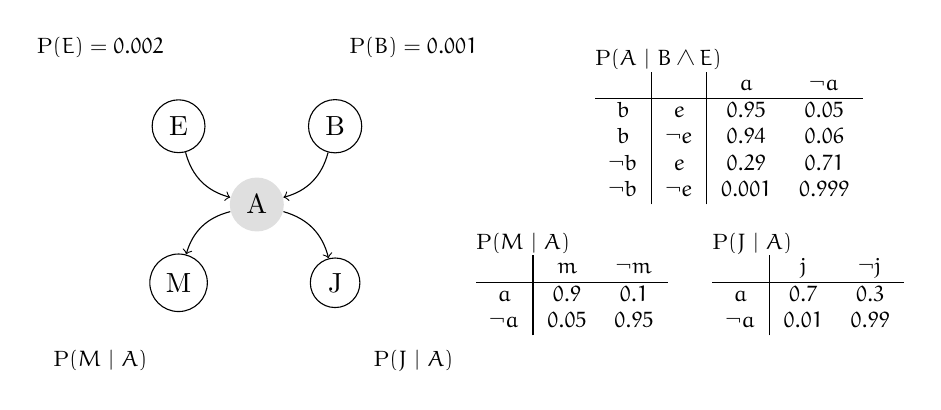
\begin{tikzpicture}[node distance=4em]

			% Nodes
			\node[smodel, circle] (A) {A};
			\node[tchoice, above left of=A] (E) {E};
			\node[above left of=E] {\footnotesize{$\pr{E}=0.002$}} ;
			\node[tchoice, above right of=A] (B) {B};
			\node[above right of=B] {\footnotesize{$\pr{B}=0.001$}} ;
			\node[tchoice, below left of=A] (M) {M};
			\node[below left of=M] {\footnotesize{$\pr{M \given A}$}} ;
			\node[tchoice, below right of=A] (J) {J};
			\node[below right of=J] {\footnotesize{$\pr{J \given A}$}} ;

			% Edges
			\draw[->] (B) to[bend left] (A);
			\draw[->] (E) to[bend right] (A);
			\draw[->] (A) to[bend right] (M) ;
			\draw[->] (A) to[bend left] (J);

			%   EDIT: fc
			%   Tables
			\node at (4,-1) {\footnotesize
				$
					\begin{aligned}
						 & \pr{M \given A}        \\[-0.55em]
						 & \begin{array}{c|cc}
									  & m    & \neg m \\
							   \hline
							   a      & 0.9  & 0.1    \\
							   \neg a & 0.05 & 0.95
						   \end{array}
					\end{aligned}
				$};
			\node at (7,-1) {\footnotesize
				$
					\begin{aligned}
						 & \pr{J \given A}        \\[-0.55em]
						 & \begin{array}{c|cc}
									  & j    & \neg j \\
							   \hline
							   a      & 0.7  & 0.3    \\
							   \neg a & 0.01 & 0.99
						   \end{array}
					\end{aligned}
				$};
			\node at (6,1) {\footnotesize
				$
					\begin{aligned}
						 & \pr{A \given B \wedge E}         \\[-0.55em]
						 & \begin{array}{c|c|cc}
									  &        & a     & \neg a \\
							   \hline
							   b      & e      & 0.95  & 0.05   \\
							   b      & \neg e & 0.94  & 0.06   \\
							   \neg b & e      & 0.29  & 0.71   \\
							   \neg b & \neg e & 0.001 & 0.999
						   \end{array}
					\end{aligned}
				$};

		\end{tikzpicture}
	\end{center}
	\caption{The Earthquake, Burglary, Alarm model}
	\label{Figure_Alarm}
\end{figure*}

We follow the convention of representing the (upper case) random
variable $X$ by the (lower case) positive literal $x$.
%
Considering the probabilities given in \cref{Figure_Alarm} we obtain
the following spe\-ci\-fi\-ca\-tion:

\begin{equation*}
	\begin{aligned}
		\probfact{b}{0.001} & ,\cr
		\probfact{e}{0.002} & ,\cr
	\end{aligned}
	\label{eq:not_so_simple_example}
\end{equation*}

For the table giving the probability $\pr{M \given A}$ we obtain the
program:

\begin{equation*}
	\begin{aligned}
		\probfact{\condsymb{m}{a}}{0.9}       & ,\cr
		\probfact{\condsymb{m}{\co{a}}}{0.05} & ,\cr
		m                                     & \leftarrow a \wedge \condsymb{m}{a},\cr
		m                                     & \leftarrow \neg a \wedge \condsymb{m}{\co{a}}.
	\end{aligned}
\end{equation*}

The latter program can be simplified (abusing notation) by writing
$\probrule{m}{0.9}{a}$ and $\probrule{m}{0.05}{\neg a}$.

Similarly, for the probability $\pr{J \given A}$ we obtain

\begin{equation*}
	\begin{aligned}
		\probrule{j}{0.7}{  & a},      \\
		\probrule{j}{0.01}{ & \neg a},
	\end{aligned}
\end{equation*}

Finally, for the probability $\pr{A \given B \wedge E}$ we obtain

\begin{equation*}
	\begin{aligned}
		\probrule{a}{0.95}{b \wedge e},      &  &  &
		\probrule{a}{0.94}{b \wedge \co{e}},\cr
		\probrule{a}{0.29}{\co{b} \wedge e}, &  &  &
		\probrule{a}{0.001}{\co{b} \wedge \co{e}}.
	\end{aligned}
\end{equation*}

One can then proceed as in the previous subsection and analyze this
example.  The details of such analysis are not given here since they
are analogous, albeit admittedly more cumbersome.

\end{document}

